
Gli effetti principali delle radiazioni su dispositivi elettronici possono essere di due categorie \cite{bib:Effetti_Radiazioni_1987}:
\begin{itemize}
	\item Danno da spostamento {(\textit{DD})}, dislocazione degli atomi dai loro siti reticolari,
	\item Ionizzazione, generazione di coppie elettrone-lacuna ($e-h$).
\end{itemize}

\subsection{Danno da spostamento}
Quando una particella (neutrone) possiede abbastanza energia tale da poter dislocare un atomo al di fuori dalla sua posizione normale all'interno reticolo, avviene il danno da spostamento (\textit{Displacement damage}); ne risulta che le caratteristiche elettroniche del materiale vengano alterate.
Inoltre, può verificarsi che l'atomo colpito generi a sua volta altri \textit{DD}, a patto che abbia abbastanza energia. L'energia minima da trasferire ad un atomo per far si che si generi un danno da spostamento nel silicio è di $20 eV$.
% Preso da Slide di Valerio Re

% Il danno da spostamento dipende dall'energia della particella, in particolare i protoni, avendo una massa maggiore, consentono di trasferire all'atomo colpito una energia maggiore \cite{bib:Effetti_Radiazioni_su_dispositivi_optoeltronici}.

\vspace*{0.5cm}

Mentre il danno da spostamento non è molto rilevante sui MOSFET, la ionizzazione può comportare variazioni dei parametri elettrici come guadagno e tensione di soglia; per questi motivi ci concentreremo solo sugli effetti della ionizzazione.

% \vspace{0.5cm}
 
% Il passaggio di una particella ionizzante all'interno della materia, comporta una perdita di energia.
% Questa dissipazione può essere formalizzata come \todo[inlinepar]{Presa da: "Radiation\_Effects\_and\_RHA\_ESA\_Course\_9-10\_May\_2017\_TID\_MP\_FINAL\_WIN.pdf" slide 5}:
% $$ \Delta E = \Delta E_{\text{elettronica}} + \Delta E_{nucleare} $$
% La \textbf{perdita di energia elettronica} è dovuta dalle interazioni con gli elettroni negli atomi, mentre la \textbf{perdita di energia nucleare} è causata dalle interazioni con i nuclei degli atomi.
% Gran parte dell'energia persa è elettronica, poiché solo occasionalmente avvengono \textit{collisioni forti} tali da creare frammenti nucleari. Pertanto la perdita di energia totale è una buona approssimazione della perdita dell'energia elettronica \cite{bib:Effetti_Radiazioni_NASA}.

\vspace{0.5cm}

\subsection{Ionizzazione}\label{cap1:ionizzazione}
La creazione di coppie $e-h$ all'interno del dispositivo MOSFET è provocata dalla ionizzazione che a sua volta è generata dal passaggio di una o più particelle che depositano una certa quantità di energia, nel materiale. Esiste una proporzionalità diretta tra il numero di coppie elettrone-lacuna e l'energia depositata da parte della particella, che collide con il dispositivo. Per esempio, nel silicio si ha una constante di $\frac{1}{3,6eV}$ mentre per il biossido di silicio è di $\frac{1}{18eV}$ \cite{bib:Effetti_Radiazioni_NASA}.


% Il passaggio di una particella all'interno della struttura del MOSFET, rilascia una certa quantità di energia provocando la ionizzazione


% Esiste una proporzionalità diretta tra il numero di coppie $e-h$ e l'\textbf{energia elettronica persa} da parte della particella che collide con il dispositivo. Per esempio, nel silicio si ha una constante di $\frac{1}{3,6eV}$ mentre per il biossido di silicio è di $\frac{1}{18eV}$ \cite{bib:Effetti_Radiazioni_NASA}.

\vspace{0.5cm}

Negli isolanti, come l'ossido di gate dei transistori MOSFET, l'effetto della ionizzazione è cumulativo. Gli elettroni liberati da una particella ionizzante si possono muovere facilmente soprattutto grazie a effetti di campo dovuti, ad esempio, a polarizzazioni.
Al contrario, le lacune sono molto meno mobili, dai 5 ai 12 ordini di grandezza inferiori, rispetto agli elettroni. La maggior parte delle lacune riesce a sopravvive alla ricombinazione con gli elettroni, creando perciò una carica positiva vicino alla giunzione $Si/SiO_2$. Un aumento della carica positiva ha come effetto la diminuzione della tensione di soglia dei MOSFET a canale P; invece negli NMOS, dopo aver subito bassi dosaggi (inferiori a $10Mrad$), si può notare un abbassamento della tensione di soglia, mentre per dosi superiori un innalzamento. Questo andamento è dato da due fattori:
\begin{enumerate}
	\item Cariche positive intrappolate nell'ossido
	\item Cariche negative presenti nelle trappole all'interfaccia\footnote{Le trappole all'interfaccia sono imperfezioni o difetti presenti alla giunzione $Si/SiO_2$ che possono intrappolare delle cariche. Queste trappole aumentano all'aumentare della dose assorbita}
\end{enumerate}
Mentre la prima provoca l'abbassamento della tensione di soglia, la seconda, all'aumentare della dose assorbita, aumenta d'intensità, sovrastando il primo effetto e incrementando la presenza di elettroni all'interfaccia con conseguente aumento della $V_{th}$.  

\vspace{0.5cm}

Un'altro effetto presente solo negli NMOS è quello della formazione di transistor parassiti \cite{effetti_radiazioni:CMOS_IC_radiation_hardening_by_design}. Questo effetto è dovuto all'aumento delle cariche positive nella \textit{shallow trench isolation} (\textit{STI}), comportando un aumento degli elettroni nel substrato (figura \ref{fig:accumulo_lacune_STI}) che, a loro volta, creano un canale conduttivo tra source e drain, aggirando quello principale. Questo collegamento fa sì che possa esserci un flusso di corrente anche quando il dispositivo è polarizzato con una $V_{GS} \simeq 0$.

\begin{figure}[ht]
	\centering

	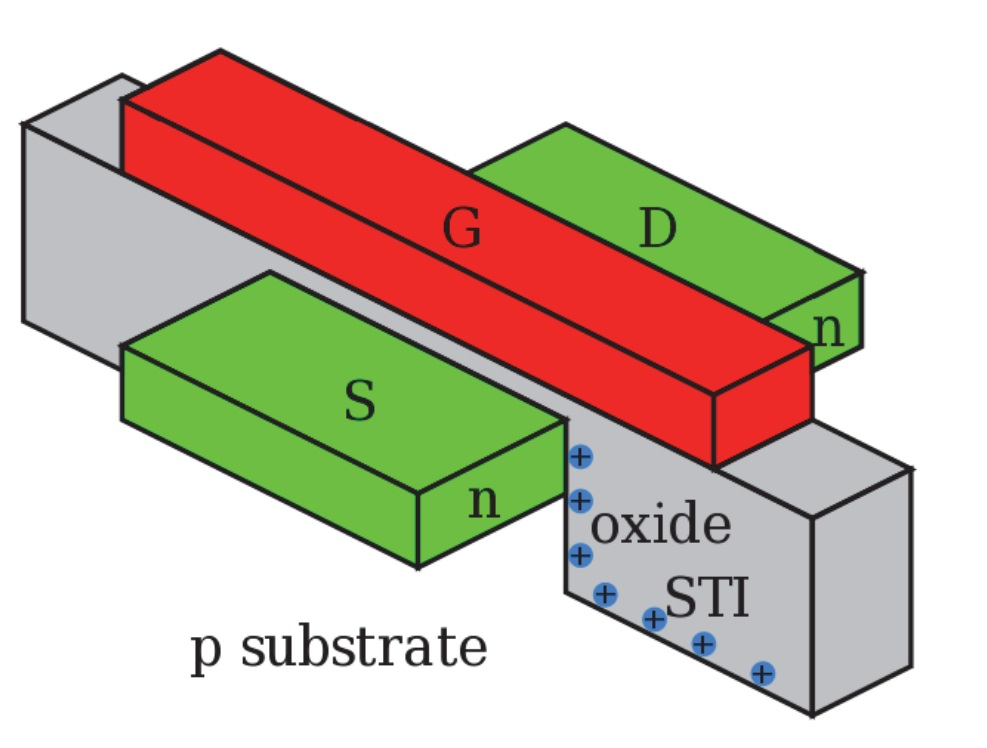
\includegraphics[width = 0.5 \textwidth]{capitolo1/effettiRadiazioniIonizzanti/Holes-trapped-in-the-shallow-trench-isolation-STI.jpg}

	\caption[Lacune nella \textit{STI}]{Accumulo delle lacune nella \textit{shallow trench isolation} \cite{effetti_radiazioni:CMOS_IC_radiation_hardening_by_design}.}
	\label{fig:accumulo_lacune_STI}

\end{figure}

Poiché gli effetti delle radiazioni sui MOSFET precedentemente elencati sono maggiori sui dispositivi a canale N, in passato si è consolidata la preferenza ad utilizzare i PMOS essendo più tolleranti alla ionizzazione. L'evoluzione di tecnologie MOSFET sempre più piccole, però, ha comportato un aumento della resistenza alle radiazioni ionizzanti, riducendo correnti di perdita, $I_{off}$ e variazioni della tensione di soglia (figura \ref{fig:scaling_mosfet}).  

\begin{figure}[ht]
	\centering

	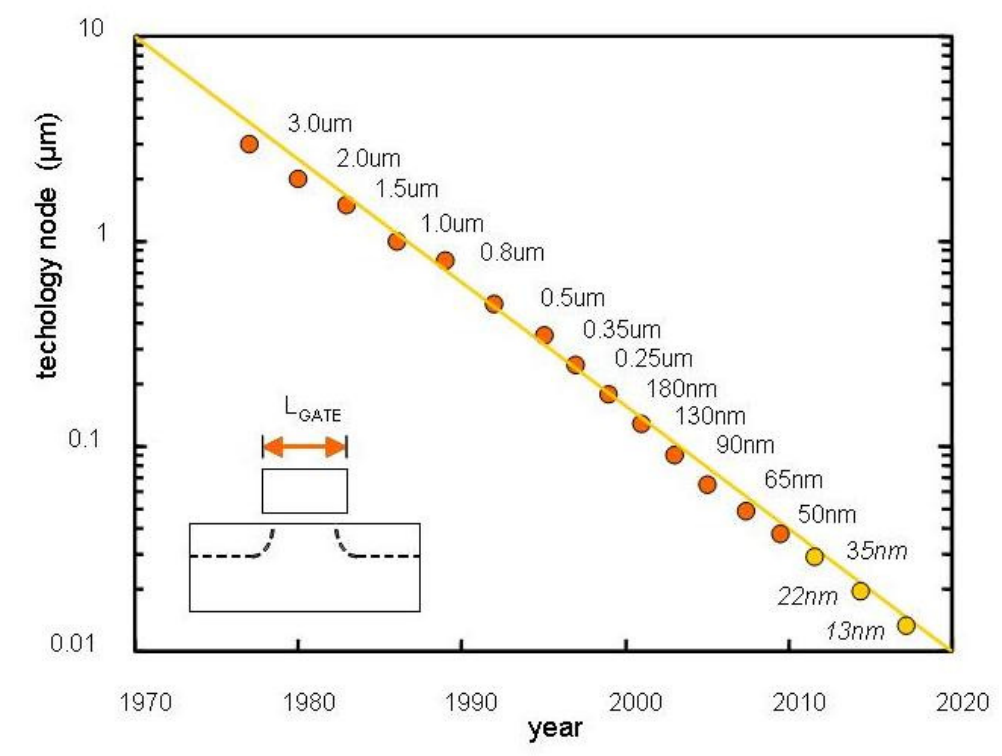
\includegraphics[width = 0.60\linewidth]{capitolo1/effettiRadiazioniIonizzanti/scaling_mosfet.png}
	\caption[Scaling dei dispositivi elettroni]{Evoluzione delle dimensioni nei dispositivi elettronici \cite{effetti_radiazioni_scaling:Nanoelectronics_and_nanolithography}}
	\label{fig:scaling_mosfet}
\end{figure}


\vspace{0.5cm}

La ricottura dell'ossido (\textit{oxide anneals}) è una procedura volta a ripristinare, almeno in parte, le caratteristiche del MOSFET a seguito dell'assorbimento di radiazioni.
Questo processo consiste nel neutralizzare le lacune scaldando il dispositivo e facendo si che gli elettroni presenti acquisiscano abbastanza energia per potersi ricombinare con le lacune. Per questo lavoro di tesi, sono stati portati ad una temperatura di $100\degree C$ per ventiquattro ore. La ricottura può avvenire anche a temperatura ambiente, ma i tempi per osservare effetti significativi sarebbero molto lunghi, anche di anni \cite{bib:Effetti_Radiazioni_NASA}. 

\subsection{Misura della dose}
La quantità di radiazioni ionizzanti assorbite da un materiale viene chiamata \textit{TID} (\textit{total ionizing dose}) ed è espressa in energia su unità di massa.
La \textit{TID} normalmente è misurata in $rad$ (\textit{radiation absorbed dose}), definito come $100 erg  = 100 \cdot 10^{-7} J$ per grammo di materiale. Un'altra unità di misura per la \textit{TID}, accolta anche dal sistema internazionale, sono i \textit{gray} ($Gy$), dove $1 Gy = 100rad = 1\frac{J}{Kg}$.
Data l'esistenza di una dipendenza tra quantità di energia persa e il materiale su cui essa si deposita, spesso insieme all'unità di misura si indica anche il materiale; ad esempio, nel caso del biossido di silicio si indica $rad(SiO_{2})$. 



